
\section{Assembly}
Digitális technika 2. tantárgy során az Intel 8085 processzor programozásához használt Assembly programozási nyelvet tanítják. Ez a fejezet erről az Assembly-ről szól.
\subsection{Tanszéki szimulátor használata}
Van egy az IIT-n fejlesztett Intel 8085 szimulátor. Ennek segítségével tetszőleges kódot tudunk futtatni egy virtuális Intel 8085 processzoron. Tetszőleges kód alatt értem, hogy bármit, ami a processzor utasításkészlete és fordítói direktívái lehetővé tesznek. \\
A tanszéki szimulátor a következő linken érhető el: \\
\url{http://topcat.iit.bme.hu/tools/i8085sim/i8085sim.cgi} \\
A szimulátor a következő módon néz ki:

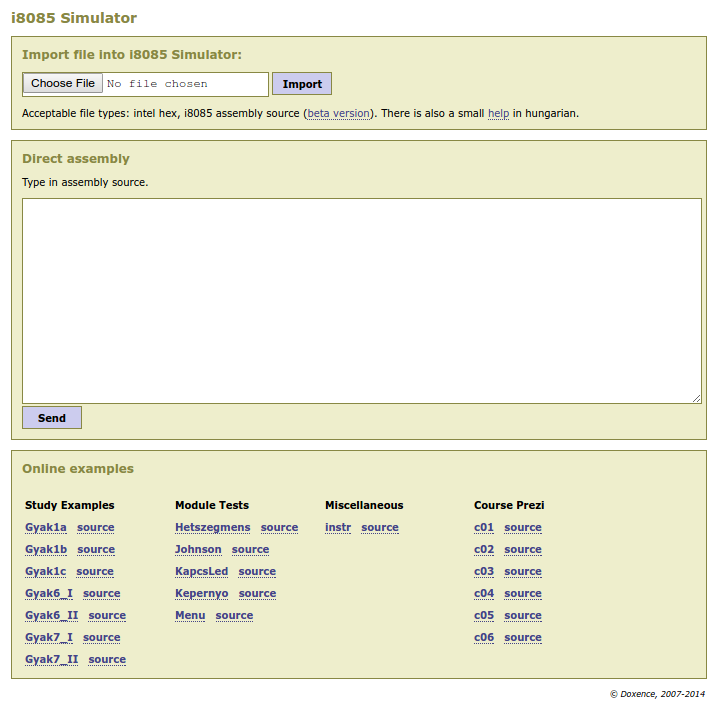
\includegraphics[scale=0.5]{sim.png} \\
A következő kódot szeretnénk a szimulátorban futtatni:
% asm kód, amit szimulálni szeretnénk
\begin{lstlisting}[frame=single]
ORG 2000h ; 2000h-tol helyezze el a kodot a fordito
LXI H, 2100h ; HL <-- 2100h
MVI M, 11h ; [2100h] = 11h
HLT ; processzor --> HALT allapot
END ; eddig forditson
\end{lstlisting}

\subsubsection{1. lépés: kód beillesztése}
A szimulálandó kódot a Direct assembly ablakba kell írni:

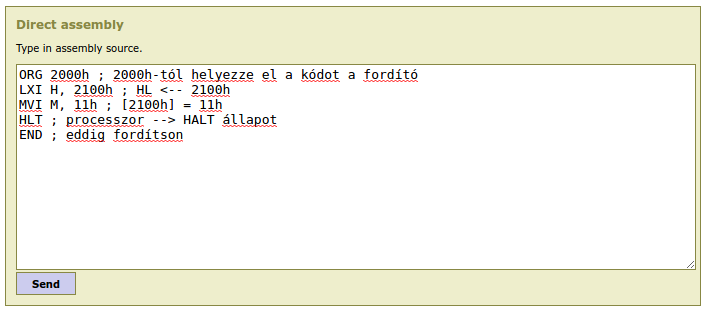
\includegraphics[scale=0.5]{sim_lepes1.png} \\
Ezután a Send gombra kattintva menjünk tovább, ahol ez fogad minket:

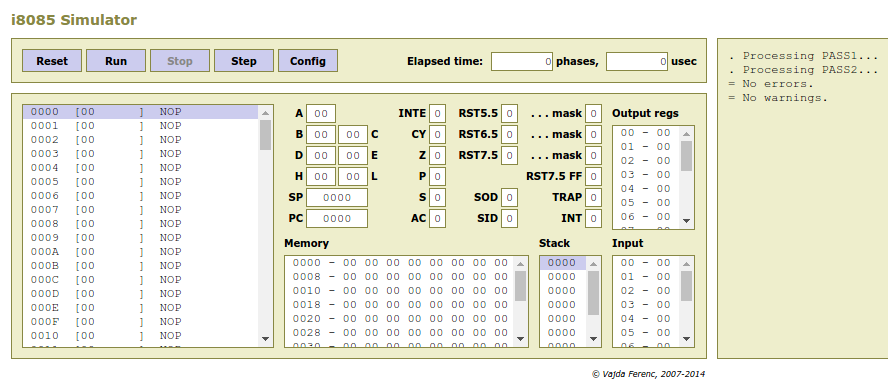
\includegraphics[scale=0.4]{sim_lepes2.png}

\subsubsection{2. lépés: szimuláció beállítása}

Néhány beállítást el kell végeznünk, hogy a megfelelő módon tudjuk nyomon követni a futó kódot.
\begin{enumerate}
  \item Coda Start at: cím, ahova elhelyezzük a kódot (és kattintsunk bele a fehér téglalapba, hogy megjelenjen ott a PC felirat)
  \item Show bus activity: legyen bepipálva
  \item Follow code: legyen bepipálva
\end{enumerate}
Az utolsó 2 opció ahhoz kell, hogy egy szép táblázatos formában jelenítse meg a kód futását és utasításonként haladjon a kód végrehajtása során.
Ezek elvégzése után ezt kell látni:

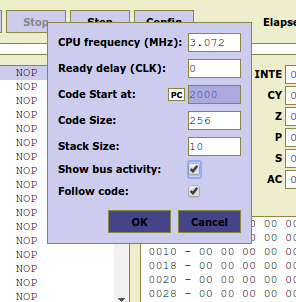
\includegraphics[scale=0.5]{sim_lepes3.png} \\
Az OK gombra kattintva megjelenik az oldal alján a táblázat fejléce:

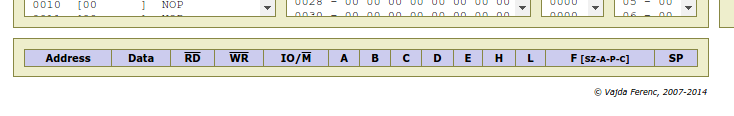
\includegraphics[scale=0.48]{sim_lepes4.png}

A táblázat fejléce:
\begin{enumerate}
  \item Address: milyen címre mutat éppen a PC
  \item Data: milyen adat van ezen a memóriacímen
  \item $\overline{RD}$: olvasás-e a jelenlegi művelet
  \item $\overline{WR}$: írás-e a jelenlegi művelet
  \item $IO/\overline{M}$: a mostani utasítás memória vagy periféria műveletet hajt végre
  \item regiszterek aktuális értékei
  \item F [SZ-A-P-C]: flag-ek aktuális értékei
  \begin{enumerate}
    \item Sign flag: előjel flag
    \item Zero flag: zérus flag
    \item Auxillary carry flag: fél-átvitel flag
    \item Parity flag: paritás flag
    \item Carry flag: átvitel flag
  \end{enumerate}
  \item SP: Stack Pointer aktuális értéke
\end{enumerate}
A PC mezőbe írjuk bele a címet, ahova helyeztük a kódot, jelen példában a 2000h-t:

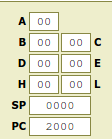
\includegraphics[scale=0.5]{sim_lepes5.png} \\
Ha be kell állítani a regiszterek kezdőértéket, akkor a megfelelő regiszterek mezőjébe írjuk bele a szükséges értéket.

\subsubsection{3. lépés: kód követése}

A bal oldali ablakban látható, hogy a PC a 2000h-ra mutat, ezt a kék háttérrel jelöli a rendszer (soron következő utasítás).\\
Ha rámegyünk a Step gombra az oldal tetején, akkor lefuttatja a PC által jelölt utasítást és az oldal alján elhelyezkedő táblázatban megjelenik néhány adat:

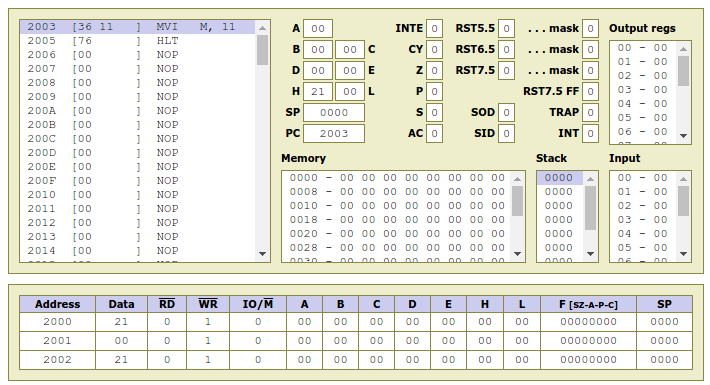
\includegraphics[scale=0.5]{sim_lepes6.png} \\
Vegyük sorra, hogy mi minden történt:
\begin{enumerate}
  \item A bal oldali fehér ablakban a kék háttér most már a soron következő utasításra mutat (MVI   M, 11), hiszen az előző utasítást már lefuttattuk és tovább lépett.
  \item A táblázatban megjelentek az LXI H, 2100h utasítás során történt dolgok.
  \begin{enumerate}
    \item Mivel a 2000h-ra helyeztük el a kódot, a PC onnan olvassa fel az első adatot. Ott egy LXI utasítás van, ezért az első adat, amit felolvas az az utasítás opkódja.
    \item \colorbox{orange!30}{Ökölszabály: minden utasítás első bájtja az opkódja.}
    \item \colorbox{orange!30}{Opkód: utasítás egyedi azonosító kódja}
    % ami alapján tudja a processzor, hogy milyen fizikai műveleteket kell elvégeznie.
    \item Az LXI utasításhoz 2 dolog tartozik még: a regiszterpár, ahova adatot mozgatunk és maga az adat, amit mozgatunk. A regiszterpár az opkódba van kódolva, ezt a segédletből ki lehet olvasni. A másik paraméter, hogy milyen adatot akarunk elhelyezni a regiszterpárba. 2 bájtos adatot tudunk egy regiszterpárba tenni, ezért ez a 2 bájt az opkódot követő következő 2 címen helyezkedik el.
    \item \colorbox{orange!30}{Little-endian: kisebb címen kisebb helyiérték}
    \item a 2100h számot szeretnénk a HL regiszterekbe tenni, szóval először felolvassuk a 2100h alsó bájtját (00h) a 2001h címről, majd a felső bájtját (21h) a 2002h címről.
    \item \colorbox{orange!30}{Egy utasítás opkódja és a paraméterei címfolytonosan helyekednek el a memóriában}
    \item \colorbox{orange!30}{Címfolytonos: egymást követő memóriacímeken.}
    \item \colorbox{orange!30}{Az opkód és az utasítás paramétereinek beolvasása mind olvasás művelet.}
  \end{enumerate}
  \item A Step-re kattintva lefuttatja a jelenlegi utasítást, ami az MVI M, 11h, majd megjelennek a táblázatban az eközben történtek:
  \begin{enumerate}
    \item Címfolytosan helyezkedik el a kód, szóval a következő címen van az MVI M utasítás opkódja, vagyis a 2003h-n.
    \item Az MVI M utasításhoz tartozik egy paraméter: milyen adatot akarunk elhelyezni az M által mutatott memóriacímre. Ezt az adatot az opkódot követő címről olvassa fel, tehát a 2004h-ról.
    \item Felolvastunk az MVI M, 11h-hoz tartozó minden adatot, szóval el tudjuk ténylegesen végezni az utasítást fizikailag is: elhelyezzük az M által mutatott memóriacímre a 11h-t.
    \item Az M pointer a HL regiszterpár tartalmával jelölt memóriacímre mutat, a HL-ben jelenleg a 2100h van, hiszen az imént tettük bele. Így a 2100h címre írjuk a 11h-t. Ez látszik a táblázatban is.
    \item Figyeljük meg, hogy a $\overline{WR} = 0$, mert ez egy adat írása egy adott memóriacímre. Az Address oszlopban a 2100h szerepel, hiszen erre a címre írunk adatot. A Data oszlopban a 11h érték szerepel, mert ezt az adatot írjuk oda.
    \item \colorbox{orange!30}{A H és L oszlopokban a  regiszterpár tartalma az előbb odahelyezett 21h és 00h.}
  \end{enumerate}
  \item Ismételten a Step-re nyomva lefut a HLT utasítás is. A HLT címfolytosan helyezkedik el (hiszen nem volt például ORG direktíva vagy hasonló), tehát a 2005h-n. Az adat csupán az utasítás opkódja, mert ehhez az utasításhoz nem tartozik semmilyen paraméter sem.
  \item Végeztünk, elvileg most megtanultuk használni a szimulátort. Ezek után sok gyakorlással ezekkel az alapokkal már ügyesen fogunk tudni bánni ezzel a hasznos kis segédeszközzel.
\end{enumerate}

\subsection{Utasísátok}
\subsubsection{CALL}
A CALL utasítás egy feltétel nélküli szubrutinhívás. \\
A legfontosabb ismeretek a CALL utasítás használatához:
\begin{enumerate}
  \item Kimenti a stackre a CALL utáni utasítás címét, vagyis eltárolja a szubrutin visszatérési címét, ahonnan folytatni kell a szubrutinból való visszatérés után.
  \item A stack müvelet kapcsán csökkenti az SP tartalmát kettővel (hiszen 2 bájtot írtunk a stackre)
  \item A PC-t átállítja z utasítás 2. és 3. bájtjában kapott címre, vagyis a szubrutin címétől folytatja a program végrehajtását
  \item 5 gépi ciklus: opkód olvasás (1 ciklus), szubrutin címének felolvasása (2 ciklus), írás a stackre (2 ciklus)
\end{enumerate}
Nézzük egy példát erre. Tételezzük fel, hogy az SP értéke 9100h.
% asm kód: call utasítás
\begin{lstlisting}[frame=single]
; SP erteke: 9100h
ORG 1200h ; innentol helyezzuk el a kodot
CALL SZUBRUTIN ; szubrutinhivas
...
ORG 5000h ; szubrutin kezdocime
SZUBRUTIN:
IN 12h ; elso utasitas a szubrutinban
...
RET ; visszateres a szubrutinbol
...
\end{lstlisting}
A program futása során a következő adatok lesznek a memória- és a címsínen:
\begin{center}
\begin{tabular}{ |c|c|c|l| }
 \hline
 Cím (hexa) & Adat (hexa) & Írás / olvasás & Megjegyzés \\ \hline
 1200 & CD & olvasás & CALL opkódjának olvasása \\ \hline
 1201 & 00 & olvasás & szubrutin címének olvasása (alsó bájt) \\ \hline
 1202 & 50 & olvasás & szubrutin címének olvasása (felső bájt) \\ \hline
 90FF & 12 & írás & visszatérési cím felső bájtját írja a stackre \\ \hline
 90FE & 03 & írás & visszatérési cím alsó bájtját írja a stackre \\ \hline
 5000 & DB & olvasás & IN opkódjának olvasása \\ \hline
 ... & ... & ... & ... \\ \hline
\end{tabular}
\end{center}

\subsection{A stack (verem) működése}
A stack (verem) egy ideiglenes tároló, ahova regiszterpárok értékeit, szubrutinok visszatérési címeit tudjuk többet között eltárolni. \\
A stack tetejére a Stack Pointer (SP) mutat, ami egy speciális regiszter pár. \\
A stack-re kizárólag 2 bájtonként lehet adatot írni. \\
A stack-re írás lépései:
\begin{enumerate}
  \item A magasabb helyiértékű bájt kerül az SP-1-re
  \item Az alacsonyabbik bájt kerül az SP-2-re
  \item 2-vel csökken az SP értéke
\end{enumerate}
A stack-et használó néhány fontosabb utasítás:
\begin{enumerate}
  \item PUSH rp: regiszterpár mentése a stackre
  \item POP rp; regiszterpárba visszatöltése a stackről
  \item CALL addr: szubrutinhívás, visszatérési cím mentése a stackre
  \item RET: szubrutinból visszatérünk az őt meghívó programrészbe, visszatérési cím felolvasása a stackről
\end{enumerate}
\subsubsection{Stack Pointer inicializálása}
A Stack Pointernek kezdeti értéket például az LXI utasítással adhatunk:
% asm kód: sp inic
\begin{lstlisting}[frame=single]
LXI SP, 9100h ; SP erteke legyen 9100h
\end{lstlisting}
\subsubsection{Írás a stackre}
A stack-re el tudjuk menteni adott regiszterpár értékét, majd azt vissza is tudjuk tölteni onnan. \\
Gyakori eset, hogy egy szubrutin során használni szeretnénk valamelyik regisztert. Ha a szubrutinnak nem feladata a regiszterek módosítása, tehát nem ott akar például visszatérési értéket visszaadni, csak egy ideiglenes tárolóra van szükségünk, akkor a következő a teendő:
\begin{enumerate}
  \item Használni kívánt regiszterpár kimentése a stackre (PUSH utasítás)
  \item Regisztertár használata, mint ideiglenes tároló
  \item Használat után a regiszterpár eredeti értékének visszatöltése
\end{enumerate}

Nézzük erre egy példát:
\begin{lstlisting}[frame=single]
FOPROGRAM:
...
LXI SP, 9100h ; SP erteke legyen 9100h
...
CALL SZUBRUTIN ; szubrutin hivasa a foprogrambol
...
SZUBRUTIN:
PUSH D ; D regiszterpar elmentese a stack-re
LXI D, 1234h ; D regiszterpar hasznalata
...
POP D ; hasznalat utan az eredeti ertek visszatoltese
RET ; visszateres a foprogramba
\end{lstlisting}
\colorbox{orange!30}{POP-nál a megfelelő helyre mutasson az SP, különben nem a D eredeti értékét tölti vissza!}

\subsubsection{Olvasás a stackről}
A stackről 2 bájtonként lehet az adatokat visszatölteni. \\
A stackről olvasás folyamata:
\begin{enumerate}
  \item Felolvassuk az alacsonyabbik bájtot az SP által mutatott címről
  \item Felolvassuk a magasabbik helyiértékű bájtot az SP+1 címről
  \item Megnöveljük 2-vel az SP értékét
\end{enumerate}

\subsubsection{Példa a stack műveletekre}
Vizsgáljuk meg az alábbi kódot.
\begin{lstlisting}[frame=single]
FOPROGRAM:
...
LXI SP, 9100h ; SP erteke legyen 9100h
LXI D, 1234h ; DE regiszterpar erteke legyen 1234h
...
ORG 1000h ; innentol helyezzuk el a kodot
CALL SZUBRUTIN ; szubrutin hivasa a foprogrambol
...
ORG 2000h ; innentol helyezzuk el a kodot
SZUBRUTIN:
PUSH D ; D regiszterpar elmentese a stack-re
...
ORG 2010h ; innentol helyezzuk el a kodot
POP D ; hasznalat utan az eredeti ertek visszatoltese
RET ; visszateres a foprogramba
\end{lstlisting}
A program futása során a következő adatok lesznek a memória- és a címsínen:
\begin{center}
\begin{tabular}{ |c|c|c|c| }
 \hline
 Cím (hexa) & Adat (hexa) & Írás / olvasás & Megjegyzés \\ \hline
 1000 & CD & olvasás & CALL opkódjának olvasása \\ \hline
 1001 & 00 & olvasás & szubrutin címének olvasása (alsó bájt) \\ \hline
 1002 & 20 & olvasás & szubrutin címének olvasása (felső bájt) \\ \hline
 90FF & 10 & írás & visszatérési cím felső bájtját írja a stackre \\ \hline
 90FE & 03 & írás & visszatérési cím alsó bájtját írja a stackre \\ \hline
 2000 & D5 & olvasás & PUSH D opkódjának olvasása \\ \hline
 90FD & 12 & írás & D regiszter tartalmat menti az SP-1-re \\ \hline
 90FC & 34 & írás & E regiszter tartalmat menti az SP-2-re \\ \hline
 ... & ... & ... & ... \\ \hline
 2010 & D1 & olvasás & POP D opkódjának olvasása, visszatoltes a DE-be \\ \hline
 90FC & 34 & írás & E regiszterbe visszatolti az SP-2-n levo adatot \\ \hline
 90FD & 12 & írás & D regiszterbe visszatolti az SP-1-n levo adatot \\ \hline
 2011 & C9 & olvasás & RET opkódjának olvasása \\ \hline
 90FE & 03 & olvasás & visszatérési cím alsó bájtját olvassa a stackről \\ \hline
 90FF & 10 & olvasás & visszatérési cím felső bájtját olvassa a stackről \\ \hline
 ... & ... & ... & ... \\ \hline
\end{tabular}
\end{center}

\subsection{Példa feladat az ellenőrző kérdések közül}
Tipikus vizsga példa a fordítói direktivák számonkérésére. Ennek egy rövidebb változata beugróban is gyakran szerepel.
Az értelmezend kód:

% asm kód, amit szimulálni szeretnénk
\begin{lstlisting}[frame=single]
ADAT0 EQU 14
ORG 800h
ADAT1: DB ADAT0, 11100111b
ORG 5678h
ADAT2: DS 2
ADAT3: DW 2017h
ADAT4: DW ADAT2
ADAT5: DB 314h
\end{lstlisting}
A megoldás:

\begin{center}
\begin{tabular}{ |c|c| }
 \hline
 Cím (hexa) & Adat (hexa) \\ \hline
 0800 & 0E \\ \hline
 0801 & E7 \\ \hline
 5678 & X \\ \hline
 5679 & X \\ \hline
 567A & 17 \\ \hline
 567B & 20 \\ \hline
 567C & 78 \\ \hline
 567D & 56 \\ \hline
 567E & 14 \\ \hline
\end{tabular}
\end{center}
Ez mind szép és jó, na de miért ez a megoldás? Vegyük sorra, hogy mi és miért így szerepel a megoldásban:
\begin{itemize}
  \item Az EQU fordítói direktíva egy konstans számértéket deklarál, amit az ADAT0 névvel érhetünk el. A konstans szám mögött nem szerepel számrendszert meghatározó betű, ezért alapértelmezettként decimális számrendszerben értelmezzük. Mivel a táblázat hexában kéri az adatokat, ezért a 14 decimális számot át kell váltani hexadecimális számrendszerbe, ez ugyebár az Eh lesz. Mivel bájtos szervezésű a memória, ezért ki kell egészíteni a félbájtos Eh számot bájtosra, ami egy nullás hexa számjegy eléírását jelenti.
  \item \colorbox{orange!30}{Egy bináris szám elejére tetszőleges számú nullát odaírva nem változik a szám értéke.}
  \item Az ORG fordítói direktíva azt jelenti, hogy a fordító milyen memóriacímre kezdje el elhelyezni az ORG-ot követő utasításokat a memóriában. Az ORG 800h azt jelenti tehát, hogy 0800h-tól kezdi el a kódokat elhelyezni a memóriában.
  \item \colorbox{orange!30}{A 8085-nek 16 adatvezetéke van, vagyis egy memóriacímet 4 hexa számjeggyel írunk le.}
  \item Az ORG után különböző adatokat definálunk többféle módon a fordító segítségével.
  \begin{itemize}
    \item DS (Define Space, inicializálatlan helyfoglalás): helyet foglal, de nem tölti fel tartalommal
    \item DB (Define Byte, inicializált 1 bájtos helyfoglalás): 1 bájtnyi helyet foglal és feltölti tartalommal
    \item DW (Define Word, inicializált 2 bájtos helyfoglalás): 2 bájtnyi helyet foglal és feltölti tartalommal
  \end{itemize}
  \item Az ORG után először DB szerepel, vagyis a 0800h címtől el fogunk helyezni 2 darab 1 bájtos adatot, mert a DB után 2 érték szerepel.
  \item Először a DB ADAT0 jelentését vizsgáljuk meg. Az ADAT0 konstant érték az E0h, ez pont 1 bájt, vagyis a DB trükkök nélkül el tudja helyezni a 0800h címre.
  \item a DB utáni második paraméter a következő címre (mert nem írtunk semmit, ami ezen változtatna) helyezi el az 1110111b-t. Hexába ezt át kell váltani: E7h.
  \item Még egy ORG jön, vagyis most máshova fogjuk már folytatni a kód elhelyezését, még pedig az 5678h címtől.
  \item A DS 2 jelentése, hogy 2 bájtnyi adatot fogunk inicializálás nélkül elhelyezni.
  \item \colorbox{orange!30}{A DS után szereplő számnak megfelelő bájtot foglalunk le iniciaizálás nélkül.}
  \item a DW mivel 2 bájtot helyez el, ezért 2 memóriacímre fog adatot tenni. Címfolytosan csináljuk ezt, mert nem volt újabb ORG vagy ilyesmi, ami ezen változtatna.
  \item A 2017h-t kell elhelyezni a memóriában. Ez könnyű, hiszen ez pont 2 bájt, vagyis semmi trükk. Mivel little-endian a processzor, ezért a kisebb címre az alsó bájtot tesszük, a nagyobb címre a felső bájtot. Vagyis a 17h-t az 567Ah-ra, a 20h-t az 567Bh-ra.
  \item \colorbox{orange!30}{Figyeljetek oda, hogy 09h után 0Ah van!}
  \item A következő DW-nek az ADAT2h-nek megfelelő értéket kell a memóriába tennie. Ez már picit bonyolult. Az ORG 5678h után szerepel az ADAT2 címke, tehát az ADAT2 értéke az a szám, amelyik memóriacímet jelenti ez a címke: 5678h. Ez egy 2 bájtos adat, ezt már el tudjuk helyezni little-endian módon a következő 2 memóriacímre.
  \item A végére maradt a nyalánkság, mert a DB 314h ismét trükkös. A probléma az, hogy a DB ugyebár 1 bájtnyi adatot tud a memóriába tenni, de a 314h összesen másfél bájton fér el, tehát fél bájtot nem tud betenni a memóriába. Mivel little-endian szervezésű a processzor, ezért az alacsonyabbik bájtot (a másfél bájtos adatból) elhelyezi a megfelelő címre, a maradék részet pedig levágja, ami nem fér el 1 bájton, tehát a felső fél bájtot).
\end{itemize}
